\DocumentMetadata{tagging=on,
    tagging-setup={math/setup=mathml-SE},
    pdfstandard=ua-2,
    lang=en-US
}
\documentclass[11pt,letterpaper]{article}

\usepackage{amsmath}
\usepackage{hhline}
\usepackage{multirow}
\usepackage{hyperref}
\usepackage{tikz}

\begin{document}

\title{Lab 1\\Activity Guide}
\author{CS435}
\date{Fall 2026}
\maketitle

\section{Learning Objectives}

\begin{itemize}
    \item Understand the purpose of cluster nodes
    \item Practice running distributed Spark jobs
    \item Adjust performance of parallel programs
\end{itemize}

\section{Submission Guidelines}

Individual submission to Canvas within one hour of the end of your respective lab session. You may handwrite and scan/take a picture, edit the \LaTeX \hspace{0.25em} source, or use the built-in text editor. Grading is based on the completion of the following three tasks.

\section{Activity Tasks}

\subsection{Cluster Installation}

Once you have finished the setup guide, your cluster is ready to go. Before getting started, you will need to SSH into your namenode (refer to the README file if you're unsure). Then run the \texttt{start-master.sh} and \texttt{start-workers.sh} commands. You can use the provided \\\texttt{monitor\_all\_machines.sh} script to verify the processes are running.
\newpage

\noindent
\textbf{Question 1:} In what lab is your cluster physically located? Why might it be important to have all machines in the same room?
\textbf{Answer 1:} lab 120. Having the machines in the same room minimizes network latency and makes physical maintenance easier.
\vspace{1in}

\noindent
\textbf{Question 2:} What are your master and worker nodes? How might the responsibilities of each differ?
\textbf{Answer 2:} The master node manages the cluster, distributing tasks. The worker nodes execute the computational workloads assigned to them.
\vspace{1in}

\subsection{SparkPi Example}

For the next part, we will compute a pi approximation. Consider a circle with radius $r=1$ and a square with side length $l=2$ both centered around the origin. This is our imaginary ``dartboard.''

%\tagstructbegin{tag=Figure}
%\Description{A blue circle inside of a square outline with a red bullseye in the middle.}
\begin{center}
%\tagmcbegin{tag=Artifact}
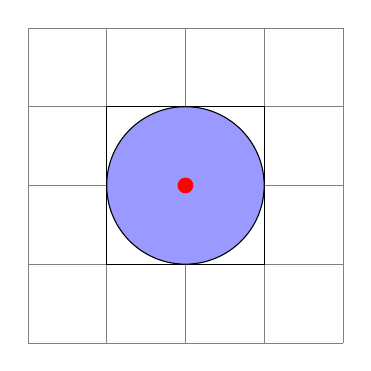
\begin{tikzpicture}
\draw[step=1cm,gray,very thin] (-2,-2) grid (2,2);
\draw (-1,-1) rectangle (1,1);
\filldraw[fill=blue!40!white, draw=black] (0,0) circle(1cm);
\fill[red] (0,0) circle(0.1cm);
\end{tikzpicture}
%\tagmcend
\end{center}
%\tagstructend

Given that $A_{\mathrm{circle}}=\pi r^2=\pi$ and $A_{\mathrm{square}}=l^2=4$, we can approximate the value of pi by randomly ``throwing darts'' and counting how many points fall inside of the circle. With enough points, $\frac{\text{points in circle}}{\text{total points}}\approx\frac{\pi}{4}$ which when multiplied by four gives us the approximation.

With that background in mind, you can now run this simulation using Apache Spark. Open the provided \texttt{SparkPi} project in IntelliJ (or your preferred IDE) and try running the code in local mode without any modifications.
\newpage
\noindent
\textbf{Question 3:} What value of pi do you get? How good is the approximation?
\vspace{1in}

Now, comment out the \texttt{.master("local")} line. This tells Spark to use distributed mode. Next, compile the program into a JAR file by running \texttt{mvn package} or using the corresponding IDE task. This can be run as a job using the command format:

\begin{verbatim}
spark-submit --class org.example.JavaSparkPi\
--master spark://<master>.cs.colostate.edu:<port>\
target/Lab1-1.0-SNAPSHOT.jar <partitions>
\end{verbatim}

You can find the master/port in the \texttt{sparkConf/spark-defaults.conf} file in your home directory. For now, you can omit the partitions argument.

\noindent
\textbf{Question 4:} Does the new value differ significantly from the previous one? Why or why not?
\vspace{1in}

\subsection{Results Discussion}

This last part is for you to experiment with the code that you have been given. Some things to consider:

\begin{itemize}
    \item How can you measure the speed of each step (and the program as a whole)?
    \item What is the effect of changing the input parameters (number of points and slices)?
    \item Are there any optimizations that can be made to the code?
\end{itemize}
\newpage
\noindent
\textbf{Question 5:} How do performing operations such as map and reduce relate to the problem itself? What does this look like in terms of how the work is distributed?
\vspace{2in}

\noindent
\textbf{Question 6:} How can you change the computation to get a better approximation? Is there a ``sweet spot'' between performance and accuracy? Can you validate this claim empirically?

\end{document}
